\section{Hexahedron}
\label{sec:Hexa}

\begin{figure}[!ht]
\begin{center}
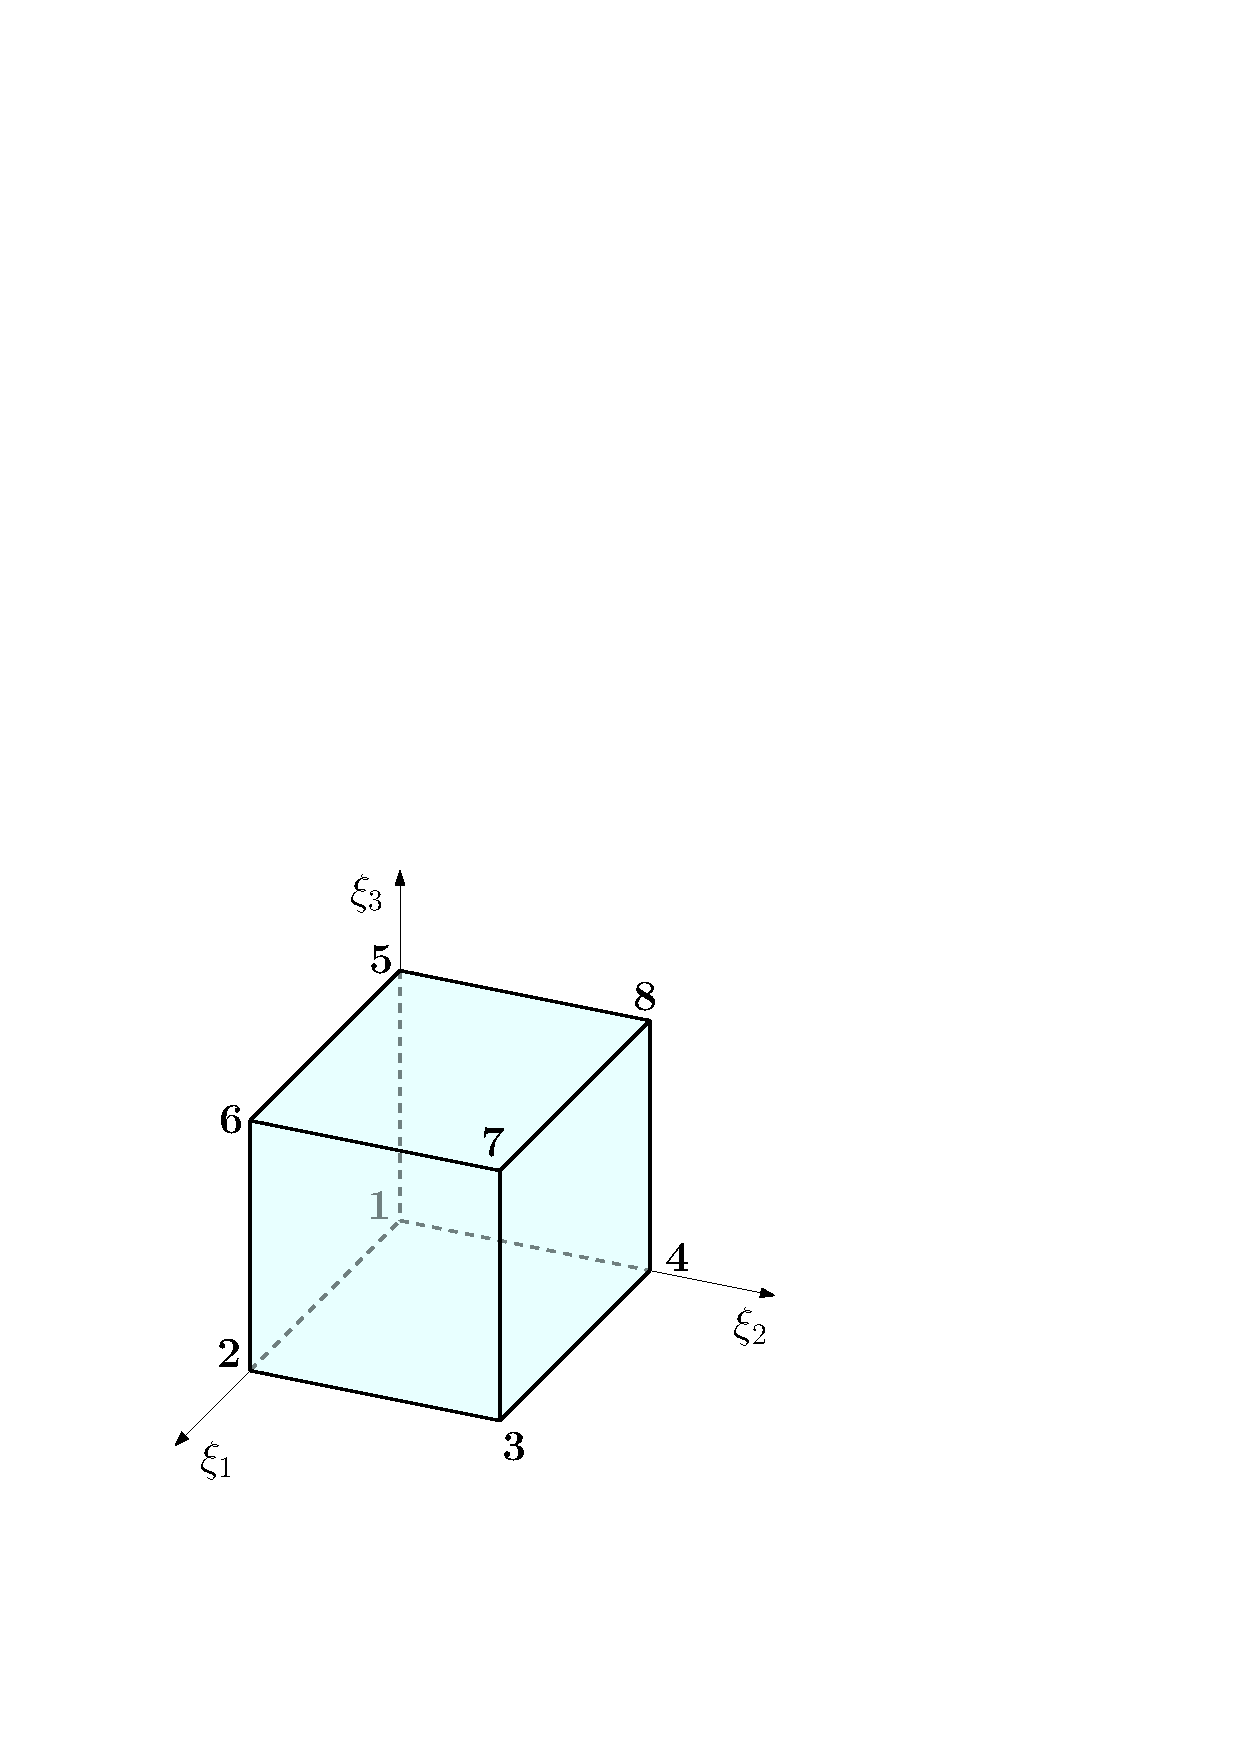
\includegraphics[scale=0.5]{./figures/MasterHexa.pdf}
\caption{Master hexahedron with numbered vertices.}
\label{fig:MasterHexa}
\end{center}
\end{figure}

The master element for hexahedra is $(0,1)^3$. 
It is shown in Figure \ref{fig:MasterHexa} in the $\xi=(\xi_1,\xi_2,\xi_3)$ space.
The master hexahedron is the Cartesian product of three segments.

%The master element for quadrilaterals is shown in Fig.~(\textit{add Figure}) in $\xi=(\xi_1,\xi_2,\xi_3)$ space.

There are \textit{three} pairs of 1D affine coordinates:
\begin{equation}
	\begin{alignedat}{4}
		\mu_0(\xi_1)&=1-\xi_1\,,\quad \mu_1(\xi_1)=\xi_1\,\qquad&\Rightarrow\qquad
			\nabla\mu_0(\xi_1)&=\bigg(\begin{smallmatrix}-1\\[2pt]0\\[2pt]0\end{smallmatrix}\bigg)\,,\quad
				\nabla\mu_1(\xi_1)=\bigg(\begin{smallmatrix}1\\[2pt]0\\[2pt]0\end{smallmatrix}\bigg)\,,\\
		\mu_0(\xi_2)&=1-\xi_2\,,\quad \mu_1(\xi_2)=\xi_2\,\qquad&\Rightarrow\qquad
			\nabla\mu_0(\xi_2)&=\bigg(\begin{smallmatrix}0\\[2pt]-1\\[2pt]0\end{smallmatrix}\bigg)\,,\quad
				\nabla\mu_1(\xi_2)=\bigg(\begin{smallmatrix}0\\[2pt]1\\[2pt]0\end{smallmatrix}\bigg)\,,\\
		\mu_0(\xi_3)&=1-\xi_3\,,\quad \mu_1(\xi_3)=\xi_3\,\qquad&\Rightarrow\qquad
			\nabla\mu_0(\xi_3)&=\bigg(\begin{smallmatrix}0\\[2pt]0\\[2pt]-1\end{smallmatrix}\bigg)\,,\quad
		\nabla\mu_1(\xi_3)=\bigg(\begin{smallmatrix}0\\[2pt]0\\[2pt]1\end{smallmatrix}\bigg)\,.
	\end{alignedat}
\end{equation}
These will be used explicitly or implicitly in the formulas that follow.

Just as with quadrilaterals, there are natural relationships between vertices, edges and faces, and the affine coordinates.
In fact, each vertex is linked to \textit{three} affine coordinates, each edge is linked to \textit{two} affine coordinates, and each face is linked to \textit{one} affine coordinate.
The linked affine coordinates take the value $1$ at the associated topological entity.
For example, vertex $1$, $v_1=(0,0,0)$, is linked to the affine coordinates $\mu_0(\xi_1)$, $\mu_0(\xi_2)$ and $\mu_0(\xi_3)$, edge 12 is linked to the affine coordinates $\mu_0(\xi_2)$ and $\mu_0(\xi_3)$, and face 1234 is linked to affine coordinate $\mu_0(\xi_3)$.

\subsubsection*{Exact Sequence}
%The three dimensional exact sequence is of the form 
%\begin{equation}
%H^1 \xrightarrow{\,\,\nabla\,\,} H(\mathrm{curl}) \xrightarrow{\nabla\times} H(\mathrm{div}) \xrightarrow{\nabla\cdot} L^2 \,.
%\label{eq:3DExactSeq}
%\end{equation}

Recall the 3D exact sequence for simply connected domains \eqref{eq:3D_exact_sequence}.
The corresponding discrete polynomial exact sequence is of the form 
\begin{equation}
	W^{p,q,r} \xrightarrow{\,\,\nabla\,\,} Q^{p,q,r} \xrightarrow{\nabla\times} V^{p,q,r} \xrightarrow{\nabla\cdot} Y^{p,q,r} \,,
\end{equation}
where the standard N\'{e}d\'{e}lec's spaces \cite{Nedelec80} of the first type for the hexahedron are utilized:
\begin{equation}
	\begin{aligned}
	W^{p,q,r} & = \mathcal{Q}^{p,q,r}= \mathcal{P}^p(\xi_1)\otimes \mathcal{P}^q (\xi_2)\otimes \mathcal{P}^r (\xi_3)\,,\\
	Q^{p,q,r} & = \mathcal{Q}^{p-1,q,r} \times\mathcal{Q}^{p,q-1,r}\times \mathcal{Q}^{p,q,r-1}\,,\\
	V^{p,q,r} & = \mathcal{Q}^{p,q-1,r-1} \times\mathcal{Q}^{p-1,q,r-1}\times \mathcal{Q}^{p-1,q-1,r}\,,\\
	Y^{p,q,r} & = \mathcal{Q}^{p-1,q-1,r-1}\,.
	\end{aligned}
\end{equation}
%Again, we follow the construction of Ainsworth and Coyle\cite{AinsworthCoyle01} based on mimicking the structure of \Nedelec's spaces with Legendre and Lobatto (integrated Legendre) polynomials. The ideas are simply extrapolated from the quadrilateral case.
As with the quadrilateral, there is a natural anisotropy of the element, which has order $p$ in the $\xi_1$ direction, $q$ in the $\xi_2$ direction and $r$ in the $\xi_3$ direction. 
The hierarchy should be maintained in $p$, $q$ and $r$ separately.  
It will sometimes be convenient to refer to $p_a$ as the order in the $\xi_a$ direction, so that $p_1=p$, $p_2=q$ and $p_3=r$.


\subsection{\texorpdfstring{$H^1$}{H1} Shape Functions}
%Recall that in three dimensions, the trace of $H^1$ functions is the value of the function itself along the boundary. 
%Hence, vertex functions should vanish at all nonadjacent faces, edge functions should vanish at all nonadjacent faces, face functions should vanish at all other faces, and bubbles should vanish at all faces. 
It will be clear that the $(p+1)(q+1)(r+1)$ shape functions defined in this section lie in $\mathcal{Q}^{p,q,r}$ and span the space.

The ideas in this section are the same as with the quadrilateral (see \S\ref{sec:Quad}) but in three dimensions.
This will simply translate to adding an extra blending function to account for the extra dimension.
Hence, the trace properties will not be analyzed in detail as they easily follow.

\subsubsection{\texorpdfstring{$H^1$}{H1} Vertices}
%First note there are three pairs of 1D affine coordinates:
%\begin{equation}
%	\begin{alignedat}{4}
%		\mu_0(\xi_1)&=1-\xi_1\,,\quad \mu_1(\xi_1)=\xi_1\,,\qquad&\Rightarrow\qquad
%			\nabla\mu_0(\xi_1)&=\bigg(\begin{smallmatrix}-1\\0\\0\end{smallmatrix}\bigg)\,,\quad
%				\nabla\mu_1(\xi_1)=\bigg(\begin{smallmatrix}1\\0\\0\end{smallmatrix}\bigg)\\
%		\mu_0(\xi_2)&=1-\xi_2\,,\quad \mu_1(\xi_2)=\xi_2\,,\qquad&\Rightarrow\qquad
%			\nabla\mu_0(\xi_2)&=\bigg(\begin{smallmatrix}0\\-1\\0\end{smallmatrix}\bigg)\,,\quad
%				\nabla\mu_1(\xi_2)=\bigg(\begin{smallmatrix}0\\1\\0\end{smallmatrix}\bigg)\\
%		\mu_0(\xi_3)&=1-\xi_3\,,\quad \mu_1(\xi_3)=\xi_3\,,\qquad&\Rightarrow\qquad
%			\nabla\mu_0(\xi_3)&=\bigg(\begin{smallmatrix}0\\0\\-1\end{smallmatrix}\bigg)\,,\quad
%		\nabla\mu_1(\xi_2)=\bigg(\begin{smallmatrix}0\\0\\1\end{smallmatrix}\bigg)\,.
%	\end{alignedat}
%\end{equation}
%These will be used explicitly or implicitly in the formulas that follow.
%The vertex functions will be products of these:
Without any delays, the vertex shape functions and their gradient are
\begin{equation}
	\begin{aligned}
		\phi^\mathrm{v}(\xi)&=\mu_a(\xi_1)\mu_b(\xi_2)\mu_c(\xi_3)\,,\\
		\nabla\phi^\mathrm{v}(\xi)&=\mu_a(\xi_1)\mu_b(\xi_2)\nabla\mu_c(\xi_3)+\mu_c(\xi_3)\mu_a(\xi_1)\nabla\mu_b(\xi_2)
			+\mu_b(\xi_2)\mu_c(\xi_3)\nabla\mu_a(\xi_1)\,,
	\end{aligned}
\end{equation}
for $a=0,1$, $b=0,1$ and $c=0,1$. 
There are a total of $8$ vertex functions (one for each vertex).

%Their gradients are
%\begin{equation}
%	\nabla\phi^\mathrm{v}(\xi)=\mu_a(\xi_1)\mu_b(\xi_2)\nabla\mu_c(\xi_3)+\mu_c(\xi_3)\mu_a(\xi_1)\nabla\mu_b(\xi_2)
%		+\mu_b(\xi_2)\mu_c(\xi_3)\nabla\mu_a(\xi_1)\,.
%\end{equation} 
%As required they vanish at all vertices except the one with coordinates $(a,b,c)$. 
%By linearity this means they also vanish at all nonadjacent edges and faces.
%Moreover, their traces over adjacent edges are of the form $\mu_b(\xi_a)$ for some $a=1,2,3$ and $b=0,1$, which coincides with the segment case. 
%The same applies to the traces over adjacent faces, which coincide with the quadrilateral face. 
%This makes the traces compatible with any potential neighboring element.
%
%Throughout the rest of this section $\vec{\mu}_{01}(\xi_a)=(\mu_0(\xi_a),\mu_1(\xi_a))$ for $a=1,2,3$, while $p_a$ is the order in the $\xi_a$ axis. That is $p_1=p$, $p_2=q$ and $p_3=r$.

\subsubsection{\texorpdfstring{$H^1$}{H1} Edges}

Again, this is analogous to the quadrilateral case, but with an extra blending function. 
Take for example edge 12.
Then, the shape functions are
\begin{equation*}
	\phi_i^\mathrm{e}(\xi)=\underbrace{\mu_0(\xi_3)\mu_0(\xi_2)}_{\text{blend}}
		 \underbrace{\phi_i^\E(\underbrace{\vec{\mu}_{01}(\xi_1)}_{\text{project}})}_{\text{evaluate}}\,,
\end{equation*}
for $i=2,\ldots,p$. 
The projection being implied is:
\begin{equation*}
	(\xi_1,\xi_2,\xi_3)\;\longmapsto\;(\xi_1,\xi_2,0)\;\longmapsto\;(\xi_1,0,0)\,.
\end{equation*}
It is illustrated in Figure \ref{fig:HexaProjection}. 
It consists simply of finding the intersection $P''=(\xi_1,0,0)$ of the edge with the normal plane passing through the original point $P=(\xi_1,\xi_2,\xi_3)$.
Alternatively it can be interpreted in two steps.
First it is projected to the closest point $P'$ in an adjacent face, by using the normal to the face.
Once in the face, it is projected again to the desired edge using the traditional \textit{two} dimensional quadrilateral projection (see Figure \ref{fig:QuadProjection}).
%by using the normal to that face and then it is projected to the desired edge by using the normal

\begin{figure}[!ht]
\begin{center}
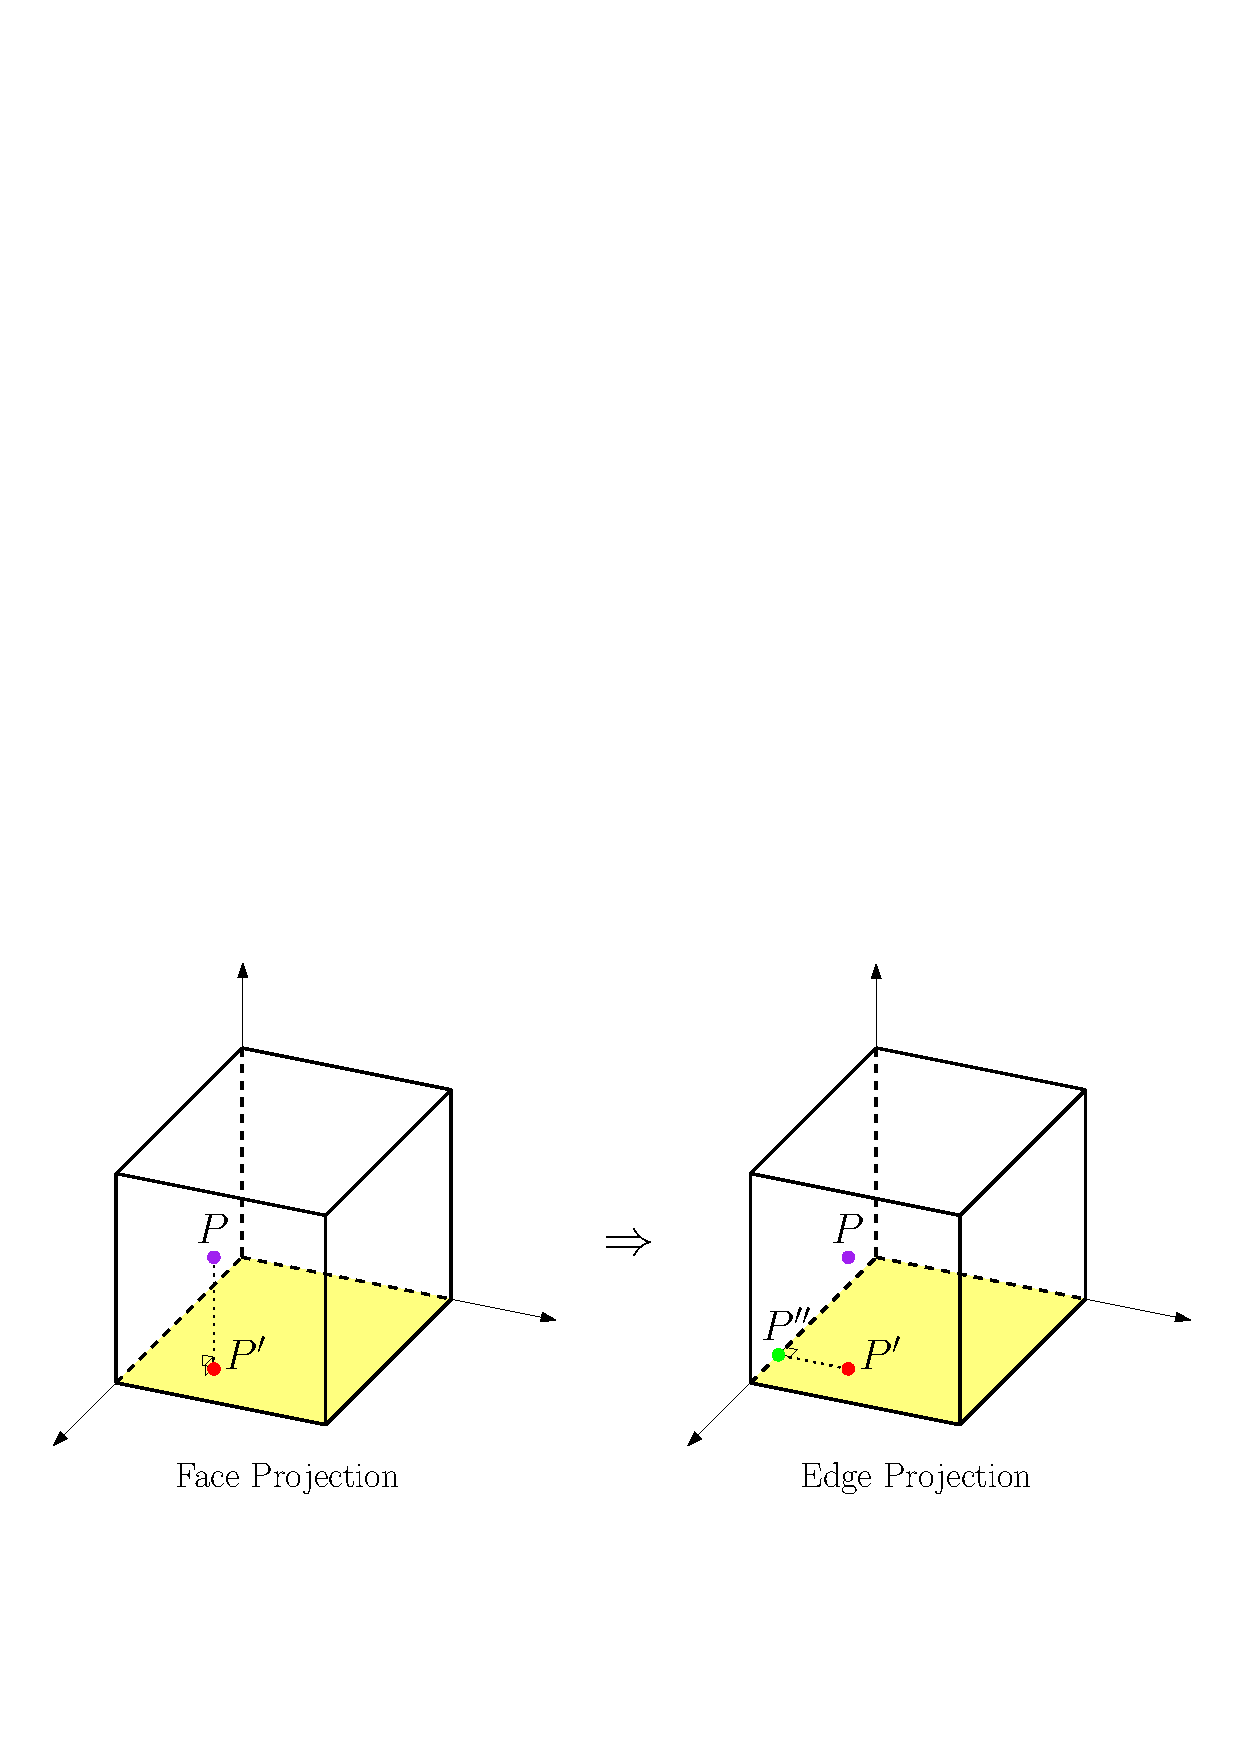
\includegraphics[scale=0.6]{./figures/HexaProjection.pdf}
\caption{Face projection from $P$ to $P'$ followed by an edge projection from $P'$ to $P''$.}
\label{fig:HexaProjection}
\end{center}
\end{figure}

%One can readily check that the required vanishing conditions and trace properties are satisfied over edges and faces.

%Again, there is an edge projection (in three dimenions) being implied:
%\begin{equation*}
%	(\xi_1,\xi_2,\xi_3)\;\longmapsto\;(\xi_1,0,0)\,.
%\end{equation*}
%It consists simply of finding the intersection $P'=(\xi_1,0,0)$ of the edge with the normal plane passing through the original point $P=(\xi_1,\xi_2,\xi_3)$. 
%This is illustrated in Fig.~(\textit{add Figure}).

The general edge shape functions and their gradient are
\begin{equation}
	\begin{aligned}
		\phi_i^\mathrm{e}(\xi)&=\mu_e(\xi_c)\mu_d(\xi_b)\phi_i^\E(\vec{\mu}_{01}(\xi_a))\,,\\
		\nabla\phi_i^\mathrm{e}(\xi)&=\mu_e(\xi_c)\mu_d(\xi_b)\nabla\phi_i^\E(\vec{\mu}_{01}(\xi_a))
			+\phi_i^\E(\vec{\mu}_{01}(\xi_a))\Big(\mu_e(\xi_c)\nabla\mu_d(\xi_b)+\mu_d(\xi_b)\nabla\mu_e(\xi_c)\Big)\,,
	\end{aligned}
	\label{eq:Hexaphigeneral}
\end{equation}
where $i=2,\ldots,p_a$, $(a,b,c)=(1,2,3),(2,3,1),(3,1,2)$, $d=0,1$ and $e=0,1$.
%Their gradients are
%\begin{equation}
%	\begin{aligned}
%		\nabla\phi_i^\mathrm{e}(\xi)=\mu_e(\xi_c)\mu_d(\xi_b)\nabla\phi_i^\E(\vec{\mu}_{01}(\xi_a))
%			+\phi_i^\E(\vec{\mu}_{01}(\xi_a))\Big(\mu_e(\xi_c)\nabla\mu_d(\xi_b)+\mu_d(\xi_b)\nabla\mu_e(\xi_c)\Big)\,.
%		\end{aligned}
%\end{equation}
For example for edge 12, this would correspond to $(a,b,c)=(1,2,3)$, $d=0$, $e=0$ and $p_a=p$, for edge 23 it is $(a,b,c)=(2,3,1)$, $d=0$, $e=1$ and $p_a=q$, and so on. 
For each edge there are $p_a-1$ shape functions, leading to a total of $4(p-1)+4(q-1)+4(r-1)$ edge functions.

%\paragraph{Edge Orientations.} These are dealt with analogously to the quadrilateral edge orientations (see the note on edge orientations in \S\ref{sec:H1edgesQuad}).

\subsubsection{\texorpdfstring{$H^1$}{H1} Faces}

Again, by adding as a blending factor the associated affine coordinate the construction becomes trivial. 
For example, for face 1234, the shape functions are
\begin{equation*}
	\phi_{ij}^\mathrm{f}(\xi)=\underbrace{\mu_0(\xi_3)}_{\text{blend}}
		\underbrace{\phi_{ij}^\square(\underbrace{\vec{\mu}_{01}(\xi_1),\vec{\mu}_{01}(\xi_2)}_{\text{project}})}_{\text{evaluate}}\,,
\end{equation*}
where $i=2,\ldots,p$ and $j=2,\ldots,q$. 
The projection is already illustrated in Figure \ref{fig:HexaProjection}, and simply consists of finding the intersection $P'=(\xi_1,\xi_2,0)$ of the normal to the face that passes through the original point $P=(\xi_1,\xi_2,\xi_3)$.
%
%Now there is \textit{face} projection involved:
%\begin{equation*}
%	(\xi_1,\xi_2,\xi_3)\;\longmapsto\;(\xi_1,\xi_2,0)\,.
%\end{equation*}
%It consists of finding the intersection $P'=(\xi_1,\xi_2,0)$ of the face with the normal line passing through the original point $P=(\xi_1,\xi_2,\xi_3)$. 
%This is shown in Fig.~(\textit{add Figure}).

In general the face shape functions and their gradient are
\begin{equation}
	\begin{aligned}
		\phi_{ij}^\mathrm{f}(\xi)&=\mu_d(\xi_c)\phi_{ij}^\square(\vec{\mu}_{01}(\xi_a),\vec{\mu}_{01}(\xi_b))\,,\\
		\nabla\phi_{ij}^\mathrm{f}(\xi)&=\mu_d(\xi_c)\nabla\phi_{ij}^\square(\vec{\mu}_{01}(\xi_a),\vec{\mu}_{01}(\xi_b))
			+\phi_{ij}^\square(\vec{\mu}_{01}(\xi_a),\vec{\mu}_{01}(\xi_b))\nabla\mu_d(\xi_c)\,,
	\end{aligned}
	\label{eq:Hexaphifacegeneral}
\end{equation}
where $i=2,\ldots,p_a$, $j=2,\ldots,p_b$, $(a,b,c)=(1,2,3),(2,3,1),(3,1,2)$, and $d=0,1$.
%Their gradients are
%\begin{equation}
%	\nabla\phi_{ij}^\mathrm{f}(\xi)=\mu_d(\xi_c)\nabla\phi_{ij}^\square(\vec{\mu}_{01}(\xi_a),\vec{\mu}_{01}(\xi_b))
%		+\phi_{ij}^\square(\vec{\mu}_{01}(\xi_a),\vec{\mu}_{01}(\xi_b))\nabla\mu_d(\xi_c)\,.\label{gradfacephiHexa}
%\end{equation}
For example for face 1234, this would correspond to $(a,b,c)=(1,2,3)$, $d=0$, $p_a=p$ and $p_b=q$, for face 1265 it is $(a,b,c)=(3,1,2)$, $d=0$, $p_a=r$ and $p_b=p$, and so on. 
For each face there are $(p_a-1)(p_b-1)$ shape functions, for a total of $2(p-1)(q-1)+2(q-1)(r-1)+2(r-1)(p-1)$ face functions.
%Clearly, this construction ensures all the desired trace properties which are consistent with the quadrilateral and segment elements.

%Notice that in \eqref{eq:Hexaphifacegeneral} the functions $\phi_{ij}^\square$ and $\nabla\phi_{ij}^\square$ are explicitly used, instead of simply writing products of $\phi_i^\E$ or even more so $L_i$. 
%Writing $\phi_{ij}^\square$ is preferred, because it reflects that the formula is representative of a quadrilateral face. 
%More importantly, when orientations play a role, it is much more convenient to have the equations in this form, since the local-to-global transformation directly handles permutations of quadruples.

%how the shape functions should be coded, since $\phi_{ij}^\square$ is called in multiple occasions from the different elements (in more general settings). 
%More importantly, these simplifications should be avoided, since by the time orientations are handled, they will change depending on the orientation.
%But with $\phi_{ij}^\square$ written directly, when orientations are included, it is a simple matter of appropriately permuting the entries of $\phi_{ij}^\square$ and $\nabla\phi_{ij}^\square$ to get the right expressions. This is shown next with an example.

%\paragraph{Face Orientations.} To consider orientations, simply take a predefined $\oo=0$ orientation for a given quadrilateral face, and replace $\phi_{ij}^\square$ with $\phi_{ij}^{\square,\oo}$ (and similarly with the gradients). For example take face 1265. The first predefined local face axis for this face, $\xi_1^\mathrm{f}$, which determines the first two entries of $\phi_{ij}^{\square,\oo}$, is parallel with the master element axis $\xi_1$. The second predefined local face axis for this face, $\xi_2^\mathrm{f}$, which determines the second pair of entries in $\phi_{ij}^{\square,\oo}$, is parallel with the master element axis $\xi_3$. Now, $\xi_1^\mathrm{f}$ and $\xi_1$ point in the same direction, meaning the first two entries of $\phi_{ij}^{\square,\oo}$ are organized as $(\mu_0(\xi_1),\mu_1(\xi_1))$ (and \textit{not} $(\mu_1(\xi_1),\mu_0(\xi_1))$). The same applies to $\xi_2^\mathrm{f}$ and $\xi_3$, which also point in the same direction. This defines the $\oo=0$ orientation, so that \eqref{eq:Hexaphifacegeneral} becomes
%\begin{equation*}
%	\phi_{ij}^\mathrm{f}(\xi)=\mu_0(\xi_2)\phi_{ij}^{\square,\oo}(\mu_0(\xi_1),\mu_1(\xi_1),\mu_0(\xi_3),\mu_1(\xi_3))\,.
%\end{equation*}
%Then, depending on the orientation $\oo$ (that is, depending on the placement of the global axes $\Xi_1^\mathrm{f}$ and $\Xi_2^\mathrm{f}$), the function will take a different form. 
%It amounts to evaluating the original function $\phi_{ij}^{\square}$ but with the entries permuted in different ways. 
%To learn how to do these permutations depending on $\oo$ see \S\ref{sec:QuadFaceOrientations}. 
%As an example, assume $\oo=1$. In that case,
%\begin{equation*}
%	\phi_{ij}^\mathrm{f}(\xi)=\mu_0(\xi_2)\phi_{ij}^{\square,1}(\mu_0(\xi_1),\mu_1(\xi_1),\mu_0(\xi_3),\mu_1(\xi_3))
%		=\mu_0(\xi_2)\phi_{ij}^{\square}(\mu_1(\xi_3),\mu_0(\xi_3),\mu_0(\xi_1),\mu_1(\xi_1))\,.
%\end{equation*}
%for $i=2,\ldots,r$ and $j=2,\ldots,p$. The same applies for the gradients, and for future face functions that will follow (which will involve $E_{ij}^\square$, $E_{ij}^\square$ and $V_{ij}^\square$).

\subsubsection{\texorpdfstring{$H^1$}{H1} Interior Bubbles}

These are constructed like the face functions, but by using edge bubbles $\phi_k^\E$ instead of the linear blending factor $\mu_d$. 
This will ensure the necessary vanishing trace properties.

The interior bubbles and their gradient are
\begin{equation}
	\begin{aligned}
		\phi_{ijk}^\mathrm{b}(\xi)&=L_i(\mu_1(\xi_1))L_j(\mu_1(\xi_2))L_k(\mu_1(\xi_3))
			=\phi_{ij}^\square(\vec{\mu}_{01}(\xi_1),\vec{\mu}_{01}(\xi_2))\phi_k^\E(\vec{\mu}_{01}(\xi_3))\,,\\
		\nabla\phi_{ijk}^\mathrm{b}(\xi)&=
			\phi_{ij}^\square(\vec{\mu}_{01}(\xi_1),\vec{\mu}_{01}(\xi_2))\nabla\phi_k^\E(\vec{\mu}_{01}(\xi_3))
				+\phi_k^\E(\vec{\mu}_{01}(\xi_3))\nabla\phi_{ij}^\square(\vec{\mu}_{01}(\xi_1),\vec{\mu}_{01}(\xi_2))\,,
	\end{aligned}
\end{equation}
for $i=2,\ldots,p$, $j=2,\ldots,q$ and $k=2,\ldots,r$. 
%Their gradients are
%\begin{equation}
%\begin{aligned}
%	\nabla\phi_{ijk}^\mathrm{b}(\xi)&=\phi_{ij}^\square(\vec{\mu}_{01}(\xi_1),\vec{\mu}_{01}(\xi_2))\nabla\phi_k^\E(\vec{\mu}_{01}(\xi_3))
%		+\phi_k^\E(\vec{\mu}_{01}(\xi_3))\nabla\phi_{ij}^\square(\vec{\mu}_{01}(\xi_1),\vec{\mu}_{01}(\xi_2))\\
%	&=\begin{pmatrix}P_{i-1}(\xi_1)L_j(\xi_2)L_k(\xi_3)\\L_i(\xi_1)P_{j-1}(\xi_2)L_k(\xi_3)\\
%		L_i(\xi_1)L_j(\xi_2)P_{k-1}(\xi_3)
%		\end{pmatrix}\,.
%\end{aligned}
%\end{equation}
Clearly there will be $(p-1)(q-1)(r-1)$ interior bubbles.



\subsection{\texorpdfstring{$H(\mathrm{curl})$}{Hcurl} Shape Functions}

%The trace of $H(\mathrm{curl})$ functions is the value of the tangential component of the vector function along the boundary (the edges and faces).
%This means all edge functions should have vanishing trace at all nonadjacent faces, face functions should have zero trace at all other faces, and bubbles should have zero trace at all faces.
It will be clear that the $p(q+1)(r+1)+q(r+1)(p+1)+r(p+1)(q+1)$ linearly independent shape functions span $Q^{p,q,r}=\mathcal{Q}^{p-1,q,r}\times\mathcal{Q}^{p,q-1,r}\times\mathcal{Q}^{p,q,r-1}$ as required.

The ideas in this section are the same as with the quadrilateral but in three dimensions. 
This will simply translate to adding an extra blending function to account for the extra dimension.
The structure of projecting, evaluating and blending still holds in $H(\mathrm{curl})$, and the projections (and even the blending functions) are the same as those in $H^1$.
As with $H^1$, the analysis of the trace properties will be superfluous.

\subsubsection{\texorpdfstring{$H(\mathrm{curl})$}{Hcurl} Edges}
These will just be the quadrilateral edge functions with the extra blending factor. They are
\begin{equation}
	\begin{aligned}
		E_i^\mathrm{e}(\xi)&=\mu_e(\xi_c)\mu_d(\xi_b)E_i^\E(\vec{\mu}_{01}(\xi_a))\,,\\
		\nabla\times E_i^\mathrm{e}(\xi)&=
			\Big(\mu_e(\xi_c)\nabla\mu_d(\xi_b)+\mu_d(\xi_b)\nabla\mu_e(\xi_c)\Big)\times E_i^\E(\vec{\mu}_{01}(\xi_a))\,,
	\end{aligned}
\end{equation}
where $i=2,\ldots,p_a$, $(a,b,c)=(1,2,3),(2,3,1),(3,1,2)$, $d=0,1$ and $e=0,1$.
%Their curls are
%\begin{equation}
%	\begin{aligned}
%		\nabla\times E_i^\mathrm{e}(\xi)=
%			\Big(\mu_e(\xi_c)\nabla\mu_d(\xi_b)+\mu_d(\xi_b)\nabla\mu_e(\xi_c)\Big)\times E_i^\E(\vec{\mu}_{01}(\xi_a))\,.
%	\end{aligned}
%\end{equation}
Notice the form is very similar to that of edge $H^1$ functions. 
For each edge there are $p_a$ shape functions, giving a total of $4p+4q+4r$ edge functions. 


\subsubsection{\texorpdfstring{$H(\mathrm{curl})$}{Hcurl} Faces}

The pattern goes on, but this time with the two families.
There are a grand total of $2(p(q-1)+q(p-1))+2(q(r-1)+r(q-1))+2(r(p-1)+p(r-1))$ face shape functions.

\subparagraph{Family I:}
The shape functions and their curl are
\begin{equation}
	\begin{aligned}
		E_{ij}^\mathrm{f}(\xi)&=\mu_d(\xi_c)E_{ij}^\square(\vec{\mu}_{01}(\xi_a),\vec{\mu}_{01}(\xi_b))\,,\\
		\nabla\times E_{ij}^\mathrm{f}(\xi)&=\mu_d(\xi_c)\nabla\times E_{ij}^\square(\vec{\mu}_{01}(\xi_a),\vec{\mu}_{01}(\xi_b))
			+\nabla\mu_d(\xi_c)\times E_{ij}^\square(\vec{\mu}_{01}(\xi_a),\vec{\mu}_{01}(\xi_b))\,,
	\end{aligned}
\end{equation}
where $i=0,\ldots,p_a-1$, $j=2,\ldots,p_b$, $(a,b,c)=(1,2,3),(2,3,1),(3,1,2)$, and $d=0,1$.
%Their curls are
%\begin{equation}
%	\nabla\times E_{ij}^\mathrm{f}(\xi)=\mu_d(\xi_c)\nabla\times E_{ij}^\square(\vec{\mu}_{01}(\xi_a),\vec{\mu}_{01}(\xi_b))
%		+\nabla\mu_d(\xi_c)\times E_{ij}^\square(\vec{\mu}_{01}(\xi_a),\vec{\mu}_{01}(\xi_b))\,.
%\end{equation}
%The form is very similar to that of $H^1$ face functions. 
For each face there are $p_a(p_b-1)$ shape functions in this family.
%Clearly, this construction ensures all the desired trace properties which are consistent with the quadrilateral and segment elements.

\subparagraph{Family II:}
The shape functions and their curl are
\begin{equation}
	\begin{aligned}
		E_{ij}^\mathrm{f}(\xi)&=\mu_d(\xi_c)E_{ij}^\square(\vec{\mu}_{01}(\xi_b),\vec{\mu}_{01}(\xi_a))\,,\\
		\nabla\times E_{ij}^\mathrm{f}(\xi)&=\mu_d(\xi_c)\nabla\times E_{ij}^\square(\vec{\mu}_{01}(\xi_b),\vec{\mu}_{01}(\xi_a))
			+\nabla\mu_d(\xi_c)\times E_{ij}^\square(\vec{\mu}_{01}(\xi_b),\vec{\mu}_{01}(\xi_a))\,,
	\end{aligned}
\end{equation}
where $i=0,\ldots,p_b-1$, $j=2,\ldots,p_a$, $(a,b,c)=(1,2,3),(2,3,1),(3,1,2)$, and $d=0,1$.
Again, recall the only difference with the first family is that the entries $(\vec{\mu}_{01}(\xi_a),\vec{\mu}_{01}(\xi_b))$ and their corresponding order $(p_a,p_b)$, are permuted.
%Their curls are
%\begin{equation}
%	\nabla\times E_{ij}^\mathrm{f}(\xi)=\mu_d(\xi_c)\nabla\times E_{ij}^\square(\vec{\mu}_{01}(\xi_a),\vec{\mu}_{01}(\xi_b))
%		+\nabla\mu_d(\xi_c)\times E_{ij}^\square(\vec{\mu}_{01}(\xi_a),\vec{\mu}_{01}(\xi_b))\,.
%\end{equation}
For each face there are $p_b(p_a-1)$ shape functions in this family.

\subsubsection{\texorpdfstring{$H(\mathrm{curl})$}{Hcurl} Interior Bubbles}

These can be constructed by using $H^1$ edge bubbles $\phi_k^\E$ as blending functions instead of the linear blending $\mu_d$ in the expressions for the face shape functions.
All permutations of $(a,b,c)$ leading to linearly independent functions must be considered.
In the end, three famillies corresponding to the cyclic permutations of $(1,2,3)$ comprise the interior bubbles.
%This leads to double counting if applied to the \textit{two} families of $H(\mathrm{curl})$ face functions. 
%Hence this is only applied to the first family. 

The interior functions and their curl are
\begin{equation}
	\begin{aligned}
		E_{ijk}^\mathrm{b}(\xi)&=\phi_k^\E(\vec{\mu}_{01}(\xi_c))E_{ij}^\square(\vec{\mu}_{01}(\xi_a),\vec{\mu}_{01}(\xi_b))\,,\\
		\nabla\times E_{ijk}^\mathrm{b}(\xi)&=\phi_k^\E(\vec{\mu}_{01}(\xi_c))\nabla\!\times\!
			E_{ij}^\square(\vec{\mu}_{01}(\xi_a),\vec{\mu}_{01}(\xi_b))
				+\nabla\phi_k^\E(\vec{\mu}_{01}(\xi_c))\!\times\! E_{ij}^\square(\vec{\mu}_{01}(\xi_a),\vec{\mu}_{01}(\xi_b))\,.
%				E_{ijk}^\mathrm{b}(\xi)&=E_{ij}^\square(\vec{\mu}_{01}^{\xi_a},\vec{\mu}_{01}^{\xi_b})\phi_k^\E(\vec{\mu}_{01}^{\xi_c})\,,\\
%		\nabla\times E_{ijk}^\mathrm{b}(\xi)&=\phi_k^\E(\vec{\mu}_{01}^{\xi_c})\nabla\!\times\!
%			E_{ij}^\square(\vec{\mu}_{01}^{\xi_a},\vec{\mu}_{01}^{\xi_b})
%				+\nabla\phi_k^\E(\vec{\mu}_{01}^{\xi_c})\!\times\! E_{ij}^\square(\vec{\mu}_{01}^{\xi_a},\vec{\mu}_{01}^{\xi_b})\,.
	\end{aligned}
\end{equation}
for $i=0,\ldots,p_a-1$, $j=2,\ldots,p_b$, $k=2,\ldots,p_c$, and $(a,b,c)=(1,2,3),(2,3,1),(3,1,2)$.
%Their curls are
%\begin{equation}
%	\nabla\times E_{ijk}^\mathrm{b}(\xi)=\phi_k^\E(\vec{\mu}_{01}(\xi_c))\nabla\times E_{ij}^\square(\vec{\mu}_{01}(\xi_a),\vec{\mu}_{01}(\xi_b))
%		+\nabla\phi_k^\E(\vec{\mu}_{01}(\xi_c))\times E_{ij}^\square(\vec{\mu}_{01}(\xi_a),\vec{\mu}_{01}(\xi_a))\,.
%\end{equation}
There will be a grand total of $p(q-1)(r-1)+q(r-1)(p-1)+r(p-1)(q-1)$ interior bubble functions.

\subsection{\texorpdfstring{$H(\mathrm{div})$}{Hdiv} Shape Functions}

%The trace of $H(\mathrm{div})$ functions is the value of the normal component of the vector function along the boundary (the faces).
%This means all face functions should have vanishing trace at all other faces, and bubbles should have zero trace at all faces.
It will be clear that all shape functions lie in $V^{p,q,r}=\mathcal{Q}^{p,q-1,r-1}\times\mathcal{Q}^{p-1,q,r-1}\times \mathcal{Q}^{p-1,q-1,r}$, which has dimension $rq(p+1)+pr(q+1)+qp(r+1)$.

This is the first time that the space $H(\mathrm{div})$ is tackled in 3D.
As expected, it requires of some analysis to develop the correct structure at first, but afterwards one can proceed very similarly as the previous spaces.

\subsubsection{\texorpdfstring{$H(\mathrm{div})$}{Hdiv} Faces}

%To understand how to build shape functions in this space, one must first understand the exact sequence at the trace level, which should also be satisfied.
%As in \S\ref{sec:HcurledgesQuad}, this is better illustrated with a diagram:
%\begin{displaymath}
%	%\text{2D:}&\qquad H^1 \xrightarrow{\,\,\nabla\,\,} H(\mathrm{curl}) \xrightarrow{\nabla\times} L^2 \\
%	%\text{1D:}&\qquad H^1 \xrightarrow{\,\,\nabla\,\,} L^2\,.
%	\xymatrix{
%				{\text{3D:}} & H^1 \ar[r]^{\nabla\,\,\,\,} \ar[d]^{\mathrm{tr}} & H(\mathrm{curl}) 
%        	\ar[r]^{\,\,\nabla\times} \ar[d]^{\mathrm{tr}} & H(\mathrm{div}) \ar[r]^{\,\,\nabla\cdot} \ar[d]^{\mathrm{tr}} & L^2\\
%        {\text{2D:}} & H^1 \ar[r]^{\nabla\,\,\,\,} \ar[d]^{\mathrm{tr}} & H(\mathrm{curl}) 
%        	\ar[r]^{\,\,\nabla\times} \ar[d]^{\mathrm{tr}} & L^2\\
%        {\text{1D:}} & H^1 \ar[r]^{\nabla\,\,\,\,} & \,\,\,\,L^2\,\, }
%\end{displaymath}

First, recall from \S\ref{sec:dimensionalhierarchy} that the normal trace of the $H(\mathrm{div})$ face functions should be a 2D $L^2$ face function.
For the purposes of motivation, take for instance face 1234.
%will take the form of one of \textit{the} 1D $L^2$ edge functions over the tangential trace.
From \eqref{eq:QuadL2Functions}, the 2D $L^2$ face functions are of the form $[P_i](\vec{\mu}_{01}(\xi_1))[P_j](\vec{\mu}_{01}(\xi_2))$.
Meanwhile, the normal vector to face 1234 is $(0,0,1)=\nabla\mu_1(\xi_1)\times\nabla\mu_1(\xi_2)$.
When coupled with a blending factor, $\mu_0(\xi_3)$, representing a linear decay (like that of $H^1$), this suggests,
\begin{equation*}
    V_i^\mathrm{e}(\xi)=\mu_0(\xi_3)[P_i](\vec{\mu}_{01}(\xi_1))[P_j](\vec{\mu}_{01}(\xi_2))\,\nabla\mu_1(\xi_1)\times
    	\nabla\mu_1(\xi_2)
    		=\mu_0(\xi_3)E_i^\E(\vec{\mu}_{01}(\xi_1))\times E_j^\E(\vec{\mu}_{01}(\xi_2))\,,
\end{equation*}
for $i=0,\ldots,p-1$ and $j=0,\ldots,q-1$.
In fact, this expression makes a lot of sense, since a function normal to the face should be perpendicular to the two tangential $H(\mathrm{curl})$ edge functions. 
The cross product then seems like a natural idea.
Indeed, one can laboriously check that the desired normal trace properties are satified at all faces.
This motivates the definition of a new ancillary operator presented next.

%This way, the traces $H(\mathrm{div})$ functions should be in a two dimensional $L^2$ space. 
%For the polynomial spaces, this means the face functions should involve traces which are products of Legendre polynomials $P_i$.
%Moreover, they should go in the normal component to the face.
%
%Take for example face 1234. The previous discussion suggests a function of the form 
%\begin{equation*}
%	V_i^\mathrm{e}(\xi)=\mu_0(\xi_3)P_i(\xi_1)P_j(\xi_2)\bigg(\begin{smallmatrix}0\\0\\1\end{smallmatrix}\bigg)\,,
%\end{equation*}
%where the blending function ensures the required vanishing properties, $i=0,\ldots,p-1$ and $j=0,\ldots,q-1$. Since it is normal to the face, it can be interpreted as being orthogonal to the two perpendicular $H(\mathrm{curl})$ functions.

\begin{definition*}
Let $(s_0,s_1)$ and $(t_0,t_1)$ be two pairs of coordinates which are arbitrary functions of some spatial variable in $\R^N$, with $N=3$. Let $p_s$ be the order in the $(s_0,s_1)$ coordinates, and $p_t$ be the order in the $(t_0,t_1)$ coordinates. Then
\begin{equation}
	V_{ij}^{\square}(s_0,s_1,t_0,t_1)=E_i^\E(s_0,s_1)\times E_j^\E(t_0,t_1)\,,
\end{equation}
for $i=0,\ldots,p_s-1$ and $j=0,\ldots,p_t-1$. Their divergence, understood in $\R^N$, is
\begin{equation}
	\nabla\cdot V_{ij}^{\square}(s_0,s_1,t_0,t_1)=E_j^\E(t_0,t_1)\cdot(\nabla\times E_i^\E(s_0,s_1))
		-E_i^\E(s_0,s_1)\cdot(\nabla\times E_j^\E(t_0,t_1)) \,.
\end{equation}
\end{definition*}

Record also the next useful remark.
\begin{remark}
%Let $\mu^{(0)}$, $\mu_0^{\xi}$, $\mu_0^{\xi_1}\R^N\vec{\mu}_{01}^{\xi_1}\vec{\mu}_{01}^{\xi_2} \vec{\mu}_{01}^{\xi_2^s}\vec{\mu}_{01}^{\langle\xi_2\rangle}\vec{\mu}_{01}^{\xi_{2,\zeta}}\vec{\mu}_{01}^{\zeta,\xi_2}$.
Let $\mu_0^{(0)}=1-\mu_1^{(0)}$ and $\mu_0^{(1)}=1-\mu_1^{(1)}$, where $\mu_1^{(0)}$ and $\mu_1^{(1)}$ are arbitrary functions of some spatial variable in $\R^N$ with $N=3$, and where $p_{(0)}$ and $p_{(1)}$ are the orders in the coordinates $(\mu_0^{(0)},\mu_1^{(0)})$ and $(\mu_0^{(1)},\mu_1^{(1)})$ respectively. Then for all $i=0,\ldots,p_{(0)}-1$, and $j=0,\ldots,p_{(1)}-1$,
\begin{equation}
\begin{aligned}
	V_{ij}^\square(\mu_0^{(0)},\mu_1^{(0)},\mu_0^{(1)},\mu_1^{(1)})
		&=P_i(\mu_1^{(0)})P_j(\mu_1^{(1)})\nabla\mu_1^{(0)}\times\nabla\mu_1^{(1)}\,,\\
			\nabla\cdot V_{ij}^\square(\mu_0^{(0)},\mu_1^{(0)},\mu_0^{(1)},\mu_1^{(1)})&=0\,.
\end{aligned}
\label{eq:Vijsimplified}
\end{equation}
\end{remark}

Finally, the shape functions and their divergence are
\begin{equation}
	\begin{aligned}
		V_{ij}^\mathrm{f}(\xi)&=\mu_d(\xi_c)V_{ij}^{\square}(\vec{\mu}_{01}(\xi_a),\vec{\mu}_{01}(\xi_b))\,,\\
		\nabla\cdot V_{ij}^\mathrm{f}(\xi)&=\nabla\mu_d(\xi_c)\cdot V_{ij}^{\square}(\vec{\mu}_{01}(\xi_a),\vec{\mu}_{01}(\xi_b))\,,
%		V_{ij}^\mathrm{f}(\xi)&=\mu_d^{\xi_c}V_{ij}^{\square}(\vec{\mu}_{01}^{\xi_a},\vec{\mu}_{01}^{\xi_b})\,,\\
%		\nabla\cdot V_{ij}^\mathrm{f}(\xi)&=\nabla\mu_d^{\xi_c}\cdot V_{ij}^{\square}(\vec{\mu}_{01}^{\xi_a},\vec{\mu}_{01}^{\xi_b})\,,
	\end{aligned}	
\end{equation}
where $i=0,\ldots,p_a-1$, $j=0,\ldots,p_b-1$, $(a,b,c)=(1,2,3),(2,3,1),(3,1,2)$, and $d=0,1$.
%Their divergences are
%\begin{equation}
%	\nabla\cdot V_{ij}^\mathrm{f}(\xi)=\nabla\mu_d(\xi_c)\cdot V_{ij}^{\square}(\vec{\mu}_{01}(\xi_a),\vec{\mu}_{01}(\xi_b))\,.
%\end{equation}
There are $p_ap_b$ face functions for each face, leading to a total of $2pq+2qr+2rp$ face functions.

\subsubsection{\texorpdfstring{$H(\mathrm{div})$}{Hdiv} Interior Bubbles}
Using the same reasoning as with $H(\mathrm{curl})$ interior bubbles, there will essentially be three families of bubbles corresponding to the cyclic permutations of $(1,2,3)$.
The interior bubbles and their divergence are
\begin{equation}
	\begin{aligned}
		V_{ijk}^\mathrm{b}(\xi)&=\phi_k^\E(\vec{\mu}_{01}(\xi_c))V_{ij}^\square(\vec{\mu}_{01}(\xi_a),\vec{\mu}_{01}(\xi_b))\,,\\
		\nabla\cdot V_{ij}^\mathrm{f}(\xi)&=
			\nabla\phi_k^\E(\vec{\mu}_{01}(\xi_c))\cdot V_{ij}^\square(\vec{\mu}_{01}(\xi_a),\vec{\mu}_{01}(\xi_b))\,.
	\end{aligned}
\end{equation}
where $i=0,\ldots,p_a-1$, $j=0,\ldots,p_b-1$, $k=2,\ldots,p_c$, and $(a,b,c)=(1,2,3),(2,3,1),(3,1,2)$.
%Their divergences are
%\begin{equation}
%	\nabla\cdot V_{ij}^\mathrm{f}(\xi)=\nabla\phi_k^\E(\xi_c)\cdot V_{ij}^{\square}(\vec{\mu}_{01}(\xi_a),\vec{\mu}_{01}(\xi_b))\,.
%\end{equation}
There are a grand total of $pq(r-1)+qr(p-1)+rp(q-1)$ bubbles.

\subsection{\texorpdfstring{$L^2$}{L2} Shape Functions}


%These should span the same space as the span of the curls of the $H(\textrm{curl})$ shape functions.
As expected, they are the tensor products of the 1D $L^2$ shape functions, and there are $pqr$ such functions spanning $Y^{p,q,r}=\mathcal{Q}^{p-1,q-1,r-1}$.

\subsubsection{\texorpdfstring{$L^2$}{L2} Interior}

The coordinate free $L^2$ interior functions for the hexahedron are
\begin{equation}
    \psi_{ijk}^\mathrm{b}(\xi)=[P_i](\vec{\mu}_{01}(\xi_1))[P_j](\vec{\mu}_{01}(\xi_2))[P_k](\vec{\mu}_{01}(\xi_3))
    	(\nabla\mu_1(\xi_1)\!\!\times\!\!\nabla\mu_1(\xi_2))\!\cdot\!\nabla\mu_1(\xi_3)\,,
\end{equation}
for $i=0,\ldots,p-1$, $j=0,\ldots,q-1$ and $k=0,\ldots,r-1$. 
There are $pqr$ interior functions.
%
%These are
%\begin{equation}
%	\psi_{ijk}^\mathrm{b}(\xi)=P_i(\xi_1)P_j(\xi_2)P_k(\xi_3),
%\end{equation}
%for $i=0,\ldots,p-1$, $j=0,\ldots,q-1$ and $k=0,\ldots,r-1$. They are easily seen to span the space $Y^{p,q,r}=\mathcal{Q}^{p-1,q-1,r-1}$ which has dimension $pqr$.

\subsection{Orientations}
\label{sec:HexaOrientations}

In 3D, both edges \textit{and} faces have orientations associated to them, and they need to be considered to ensure full compatibility of shape functions along adjacent elements.
Fortunately, these issues are handled almost effortlessly due to the structure of the formulas for the shape functions, and the local-to-global permutation functions, $\sigma_\oo^\E$, $\sigma_\oo^\square$ and $\sigma_\oo^\Tri$.
In what follows, it is assumed that \S\ref{sec:fulledgeorientations}, \S\ref{sec:QuadOrientations} and \S\ref{sec:TriaOrientations} have been covered.

To construct orientation embedded shape functions, the first step is to predefine a set of \textit{local} orientations for each edge and face at the master element level.
After they are defined, these remain fixed.
The next step is to find the associated \textit{locally ordered} tuples of affine coordinates representing those local orientations.
Once these are found, the orientation embedded shape functions are merely the usual edge and face functions, but with their respective ancillary operator being precomposed with the appropriate local-to-global permutation function.
The only ``burden'' is then to find the \textit{locally ordered} tuples.
This is shown next for the hexahedron.

\begin{figure}[!ht]
\begin{center}
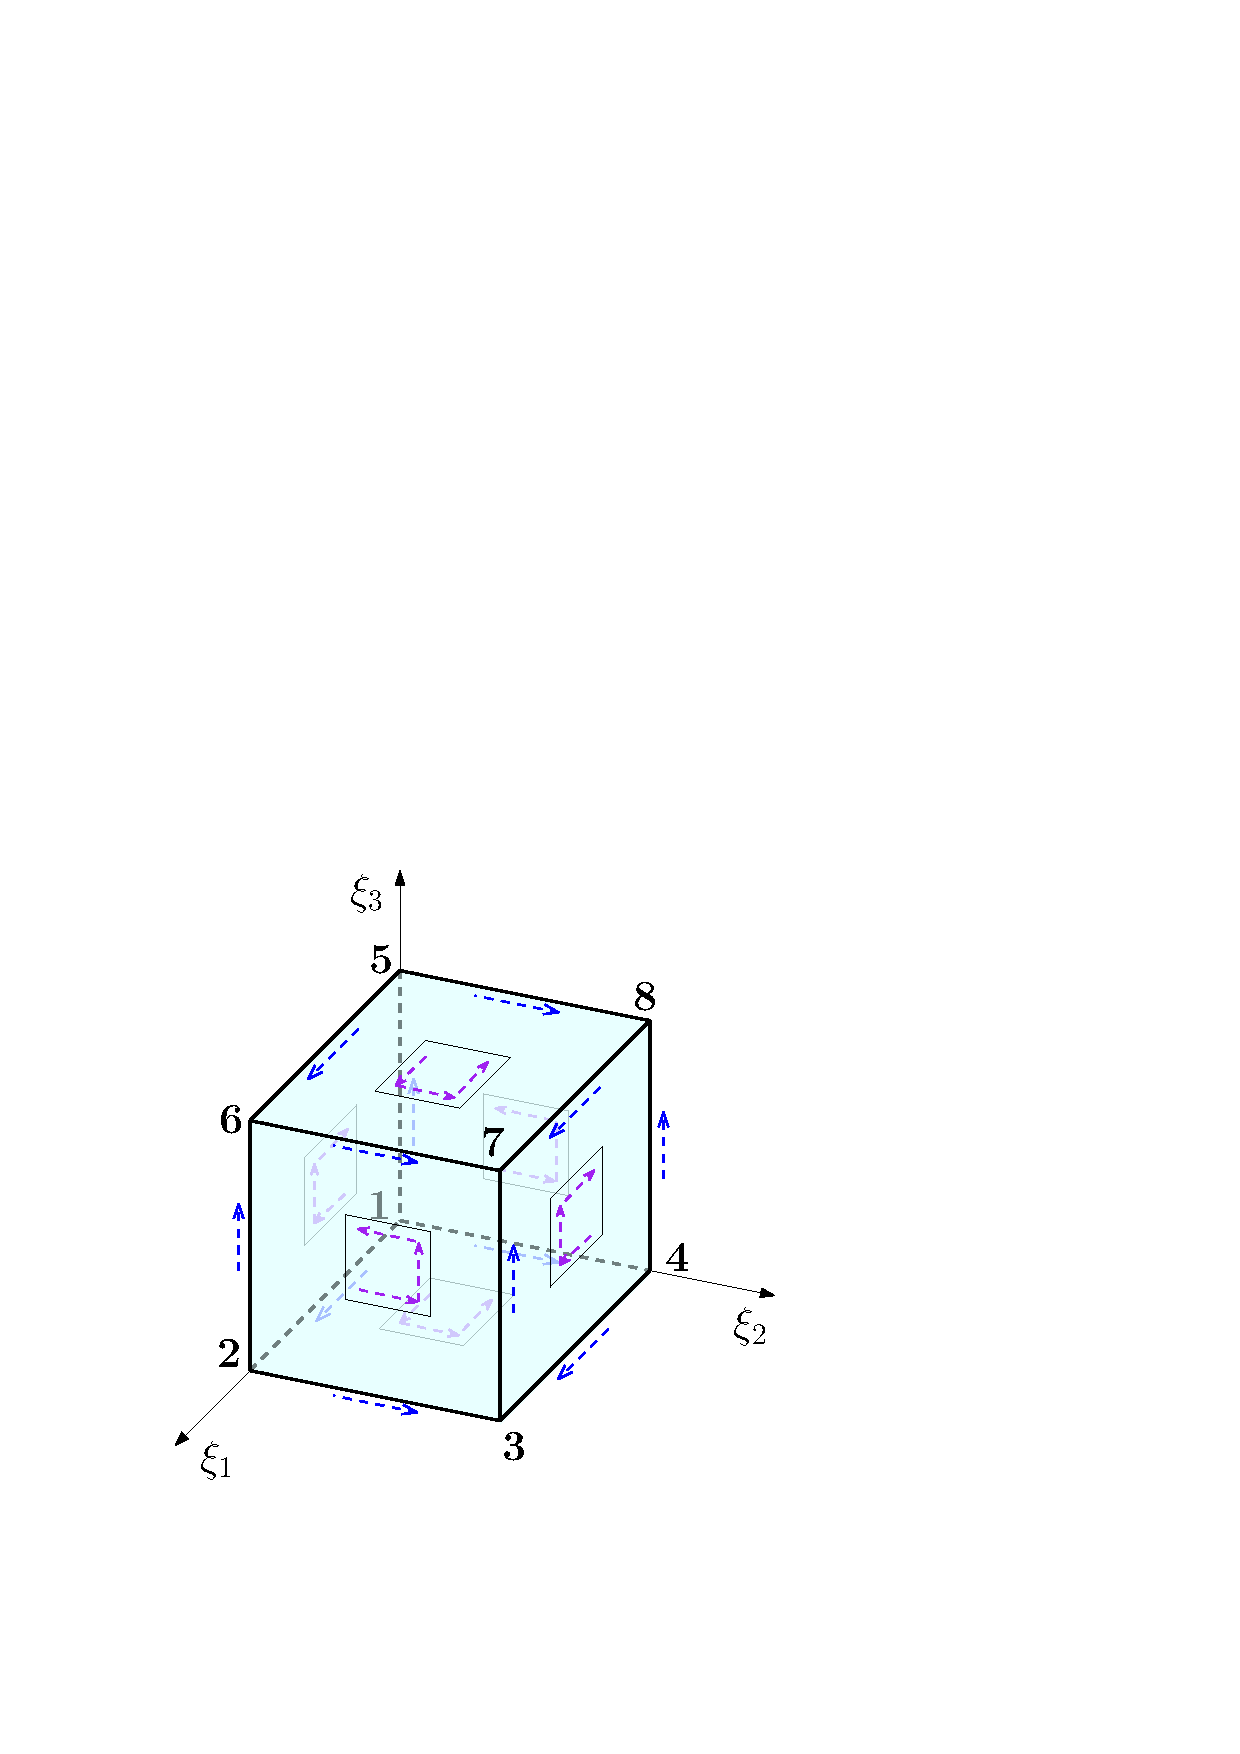
\includegraphics[scale=0.5]{./figures/MasterHexaOrientations.pdf}
\caption{Master hexahedron with numbered vertices \textit{and} local edge and face orientations.}
\label{fig:MasterHexaOrientations}
\end{center}
\end{figure}

Figure \ref{fig:MasterHexaOrientations} shows the master hexahedron along with a schematic representing all predefined \textit{local} edge and face orientations.
They represent the $\oo=0$ case.
They are \textit{our} choices for the local orientations (which in fact are the ``lexicographic'' orientations), but others may choose different local orientations to represent their $\oo=0$ case.

To find the locally ordered tuples, the key is being aware of the relationships between the vertices and the affine coordinates.
To illustrate this take as an example edge 12 and face 1234.

Edge 12 is composed of the vertices $v_1$ and $v_2$. 
Here, $v_1$ is linked to $\mu_0(\xi_1)$, $\mu_0(\xi_2)$,$\mu_0(\xi_3)$, while $v_2$ is linked to $\mu_1(\xi_1)$, $\mu_0(\xi_2)$ and $\mu_0(\xi_3)$.
The only difference between the the two vertices is that $v_1$ is linked to $\mu_0(\xi_1)$, while $v_2$ is linked to $\mu_1(\xi_1)$.
Now, the local orientation is represented by the local vertex-ordering $v_1\tdashto v_2$, so quite simply the locally ordered pair is $\vec{\mu}_{01}(\xi_1)=(\mu_0(\xi_1),\mu_0(\xi_1))$ (if the local ordering was $v_2\tdashto v_1$, then the pair would be $\vec{\mu}_{10}(\xi_1)$).
Hence, the orientation embedded edge 12 shape functions in $H^1$ with their gradient are
\begin{equation*}
	\begin{aligned}
		\phi_i^\mathrm{e}(\xi)&=\mu_0(\xi_3)\mu_0(\xi_2)\phi_i^\E(\sigma_\oo^\E(\vec{\mu}_{01}(\xi_1)))\,,\\
		\nabla\phi_i^\mathrm{e}(\xi)&=\mu_0(\xi_c)\mu_0(\xi_b)\nabla\phi_i^\E(\sigma_\oo^\E(\vec{\mu}_{01}(\xi_1)))
			+\phi_i^\E(\sigma_\oo^\E(\vec{\mu}_{01}(\xi_1)))\Big(\mu_0(\xi_3)\nabla\mu_0(\xi_2)+\mu_0(\xi_2)\nabla\mu_0(\xi_3)\Big)\,,
	\end{aligned}
\end{equation*}
where $i=2,\ldots,p$. 
The same applies to the $H(\mathrm{curl})$ edge 12 shape functions and their curl.
Clearly the approach is analogous with any other edge.

Face 1234 is composed of the vertices $v_1$, $v_2$, $v_3$ and $v_4$.
Here, the final goal is to find a locally ordered quadruple composed of two pairs.
The local vertex-ordering corresponding to the local orientation of face 1234 is $v_1\tdashto v_2\tdashto v_3\tdashto v_4$.
All one needs to do is to take the first two elements of the list, $v_1\tdashto v_2$, and the second and third components of the list, namely $v_2\tdashto v_3$.
The former will represent the \textit{first} pair in the quadruple, while the latter represent the \textit{second} pair in the quadruple.
Then one proceeds as if these where edges, so that $v_1\tdashto v_2$ is associated to $\vec{\mu}_{01}(\xi_1)$, while $v_2\tdashto v_3$ is associated to $\vec{\mu}_{01}(\xi_2)$.
Finally the locally ordered quadruple is then the ordered succession of these two pairs, $(\vec{\mu}_{01}(\xi_1),\vec{\mu}_{01}(\xi_2))$.
Hence, the orientation embedded face 1234 shape functions in $H^1$ with their gradient are
\begin{equation*}
	\begin{aligned}
		\phi_{ij}^\mathrm{f}(\xi)&=\mu_0(\xi_3)\phi_{ij}^\square(\sigma_\oo^\square(\vec{\mu}_{01}(\xi_1),\vec{\mu}_{01}(\xi_2)))\,,\\
		\nabla\phi_{ij}^\mathrm{f}(\xi)&=\mu_0(\xi_3)\nabla\phi_{ij}^\square(\sigma_\oo^\square(\vec{\mu}_{01}(\xi_1),\vec{\mu}_{01}(\xi_2)))
			+\phi_{ij}^\square(\sigma_\oo^\square(\vec{\mu}_{01}(\xi_1),\vec{\mu}_{01}(\xi_2)))\nabla\mu_0(\xi_3)\,,
	\end{aligned}
\end{equation*}
where $i=2,\ldots,p_a$, $j=2,\ldots,p_b$, where $(p_a,p_b)$ are the orders of the first and second coordinate pairs in the quadruple $\sigma_\oo^\square(\vec{\mu}_{01}(\xi_1),\vec{\mu}_{01}(\xi_2))$.
The same applies to the $H(\mathrm{curl})$ and $H(\mathrm{div})$ face 1234 shape functions and their differential forms.
Once again, the approach is analogous with any other face.